\documentclass[a4full,12pt]{article}

\title{Integrating a Category-Partition Testing Tool with Combinatorial Interaction
Testing Tool To Produce T-Way Adequate Test Frames}
\author{Andrew Graff}

%\usepackage{fullpage}
%\usepackage{epsfig}
\usepackage{graphicx}
\usepackage{xcolor}
\graphicspath{ {./images/} }

\newcommand{\eas}[1]{{\color{blue}\sf ({#1})}}
\newcommand{\ag}[1]{{\color{red}\sf ({#1})}}
\renewcommand{\topfraction}{.9}
\renewcommand{\bottomfraction}{.9}
\renewcommand{\textfraction}{.1}
\begin{document}
\maketitle
\section{Introduction}
Software is the beating heart of a lot of technology today, and defects in that software
  can be costly. Some simply print funny characters to the terminal, while some can bring
  your production to a halt for hours or even days costing thousands and even millions of
  dollars. Or perhaps a security breach which exposes your intellectual property which
  could kill your business altogether. That is why testing is such an important step in
  the process of creating defect free software. Testing software can be a difficult task
  depending on the complexity of the software itself, what kind of inputs it takes, and how
  many different functions it can perform. And there are several different approaches in how
  to do the actual testing: black-box, white-box, static analysis to name a few. We will be
  focusing on black-box testing, and more specifically generating test cases that find the
  greatest amount of defects with a realistically executable number of test cases.
  
\section{Problem Statement and Proposed Solution}
It is difficult to engineer a set of tests that adequately tests a particular piece of software
  in an acceptable amount of time. Category partitioning is a useful black-box testing method that
  helps to test systematic design with test cases. It allows the user to divide
  the inputs of the software into categories of choices. \emph{tsl} (testing specification language) is a tool
  that offers a good front-end for the category partitioning method with a formal descriptive language
  to specify those categories and choices. In addition, \emph{tsl} will generate test frames in an output file.
  However, it's weakness is that it will generate all possible permutations of the categories of choices, which
  may not run in a feasible amount of time.
  
Combinatorial interaction testing addresses the problem of the brute force approach of running all
  possible combinations of choices by offering a method for analyzing and selecting a subset of test cases
  that cover combinations of choice interations. The tool we will use for this step will be \emph{casa},
  which uses simulated annealing to select the subset of interactions between choices. Given a model file and
  constraints file as input, \emph{casa} then outputs to a file a set of combinations of options that should
  be selected together. The weakness for \emph{casa} is that the constraints are expressed in conjunctive
  normal form, which is not how a typical user would think or write in. It is much easier and more human
  readable if we could write in prepositional logic. So it can be difficult to write the constraints properly.
  Additionally, the output is a set of numbers representing each choice. It's hard to map these numbers back
  to actual choices. So some remapping is required back to the original inputs (e.g. \emph{tsl} "choices").
 
\eas{Here you should talk how you propose to solve this problem. The goal of this project is to ...}
These two methodologies and tools are separate pieces of software that require the user to generate the input
  to each tool separately. This project takes on the task of combining the user-friendly input/output components
  of \emph{tsl} and integrates them into the powerful test selection algorithm of \emph{casa}. Upon completion of
  the project, a user only needs to generate the category partition test specification input file, and an
  easy to use adequate coverage set of test frames will be generated. This will eliminate the necessity for the
  user to generate the complicated and bug prone inputs to the \emph{casa} tool and remapping of the output.
  
\section{Background}
This project builds on the work of two teams that have come up with solutions to
  two different problems. Here we will explain each of those solutions and the 
  tools created to support them.

The \emph{category-partition method} uses a formal test specification language to generate
  test case descriptions. These test case descriptions would then be used to
  create an executable software test. So how do you generate the formal test 
  specifications? Depending on the size of the software system to test, the 
  engineer may need to break the program up into smaller testable blocks. For 
  the purposes of this project, we will use a simple example of a browser's 
  settings for how to treat tabs. See figure \ref{fig:tabs_example}.
\begin{figure}[htb]
\centering
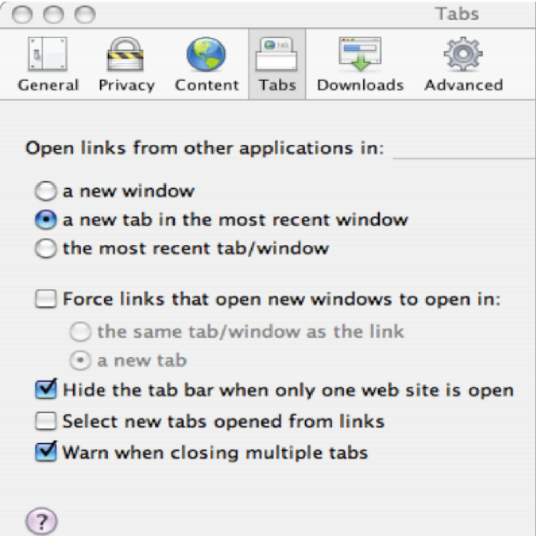
\includegraphics[width=2.3in,keepaspectratio]{images/tabs_example.png}
\caption{Sample of software feature to test tabs}
\label{fig:tabs_example}
\end{figure}

As part of the process to translate this feature into the formal language of \emph{tsl},
  we need to follow a specific format for our test specification file. It specifies
  \emph{categories}, \emph{choices}, \emph{properties}, and \emph{selectors} where 
  \emph{selectors} are boolean expressions. The format of the file looks like this:
\begin{figure}[htb]
\centering
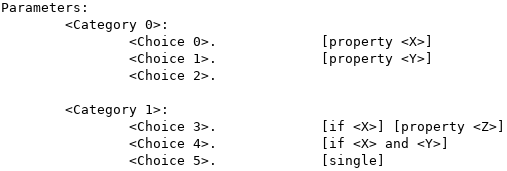
\includegraphics[width=3in,keepaspectratio]{images/tsl_format.png}
\caption{Format for tsl input file}
\label{fig:tsl_format}
\end{figure}

Back to our example, we need to choose \emph{categories} and \emph{choices} within those
  \emph{categories}. For example, one \emph{category} could be 'Link', and the choices
  associated with 'Link' are 'new window', 'new tab', and 'current tab' pulled from the
  'Open links from other applications in:' portion of the settings. We do this for all
  the available selections in this browser's 'Tabs' options. Next we assign some 
  \emph{properties}, which are useful for defining constraints that should be imposed on
  the valid \emph{choices} a program may accept. And then the \emph{selectors} are defined
  as prepositional logic statements that select the option that is associated with the 
  \emph{property} that is referenced in the \emph{selector} statement. See figure \ref{fig:tsl_input_final}.
\begin{figure}[htb]
\centering
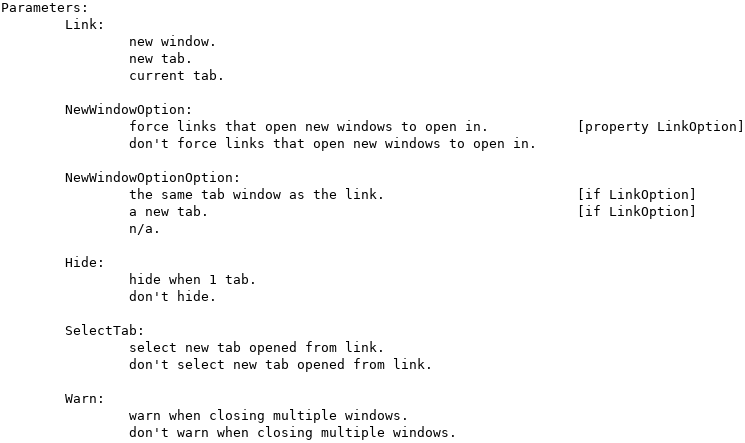
\includegraphics[width=4in,keepaspectratio]{images/tsl_input_final.png}
\caption{An input file for \emph{tsl} using our 'Tabs' example.}
\label{fig:tsl_input_final}
\end{figure}

After executing \emph{tsl} with this input file, we end up with 96 total test frames
  for all possible combinations of our 'Tabs' example. This is a small example with very
  few choices. Another, more complex system such as an airplane cockpit with many switches
  and inputs. How many possible combinations would there be to test that? Brute force is not
  feasible to test this system completely, so we look for another way we can reduce the number
  of test sets down to a feasible number. The \emph{tsl} tool itself consists of 12 files and
  1,125 lines of code and is written in C.

\emph{Combinatorial interaction testing} is a testing method that relies on the principle
  that a large portion of faults can be detected with a subset of the total number of 
  possible inputs. \emph{casa} is a tool that will find a \emph{t-way} pairwise covering 
  array that satisfies all possible values for each input within it's pair in order to find
  the minimal set of inputs to cover those faults using simulated annealing as it's algorithm.
  The tool takes two files as input: one that specifies the \emph{t-way} interaction
  level desired along with all possible inputs and one that describes constraints on those
  inputs. The output is the subset of combinations that satisfy the selected \emph{t-way}
  interaction level. This allows us to identify the subset of tests necessary to get adequate
  testing coverage. The inputs must be manually generated by the user and the constraints
  file uses conjunctive normal form, which can be difficult to translate from prepositional
  logic that we have defined in our \emph{tsl} configuration file. In addition, the output
  needs some manipulation to translate back to something useful for testing.
  
The \emph{.citmodel} input file has the following format. The first line of the file
  specifies the strength of the T-way pairs to find. The second line specifies the number
  of \emph{categories} we have broken the program into. And the third line specifies how
  many \emph{choices} within the categories we have starting from the first \emph{category} to
  the last. See figure \ref{fig:casa_citmodel_input}. Next we look at the \emph{.constraints}
  file and the contraints are written as a conjunction of disjunctions. The first line in this
  file denotes how many disjunctive clauses (constraints) will be defined for this model. Each
  conjunctive clause consists of a pair of lines, the first of which specifies how many terms
  will be in the disjunctive clause. The second line of the pair is the disjunctive clause in
  conjunctive normal form for each constraint. See figure \ref{fig:casa_constraints}.

Finally, we look at the output format from the \emph{casa} program. The first line contains
  the number of combinations generated for the given \emph{.citmodel} and \emph{.constraints}
  input followed by that number of lines, each a different input combination. Each digit in
  the combination represents the \emph{choice} from the \emph{category} in order of their
  defined input. For example, with an input of '2 3 4 5' in our \emph{.citmodel}, the first
  entry of the ouput line could contain '0' or '1'. The second entry could contain '2', '3',
  or '4'. The third entry would contain '5', '6', '7' or '8', etc. This output could be used
  to generate a test frame by associating each entry in the line with it's corresponding
  \emph{choice}. See figure \ref{fig:casa_output}. The \emph{casa} tool consists of 87 files
  with 9,139 lines of code and is written in C++.
  
\begin{figure}[htb]
\centering
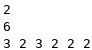
\includegraphics[width=1in,keepaspectratio]{images/casa_citmodel_input.png}
\caption{Example of \emph{casa} .citmodel input file}
\label{fig:casa_citmodel_input}
\end{figure}

\begin{figure}[htb]
\centering
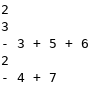
\includegraphics[width=1in,keepaspectratio]{images/casa_constraints.png}
\caption{Constraints file for our 'Tabs' example with 2 rules. If option 3 is chosen, then choose 5 or 6. If option 4 is chosen, then choose 7.}
\label{fig:casa_constraints}
\end{figure}

\begin{figure}[htb]
\centering
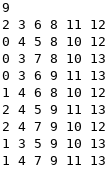
\includegraphics[width=1.25in,keepaspectratio]{images/casa_output.png}
\caption{Output from \emph{casa}}
\label{fig:casa_output}
\end{figure}

\section{Preliminary Work}
Some preliminary work has been done on this project in order to determine the
  feasibility of the idea to combine the \emph{tsl} and \emph{casa} tools into 
  a single, easy to use tool. A goal of the project is to simplify and reduce the
  effort a user needs to put in to use the new tool. Source code was acquired for
  both tools and some initial analysis of the code was done in order to understand
  how they work and where some work may be needed to combine them. As it
  turns out, the \emph{tsl} tool is written in basic C and \emph{casa} is written
  in C++. Converting \emph{tsl} to C++ would be beneficial for combining the 
  code bases into a single program. So \emph{tsl} was updated to support compilation
  with the g++ compiler.

As part of the simplification of the tool, only the category partition test specifications
  should need to be created by the user as a \emph{.tsl} file. The tool will do the rest to
  generate the adequate coverage set of test frames. Since \emph{casa} takes as input a 
  \emph{.citmodel} file, this preliminary version of \emph{tsl} generates one based on the
  specification file passed in. The generation of the \emph{.constraints} file will be created
  at a later time as part of the proposed work. In order to create the \emph{.citmodel}, we need
  to be able to keep track of the parsed information from the specifications file.
  
In order to achieve this, a new struct was added to \emph{tsl/structs.h} called \emph{container} that
  keeps track of the list of non-single Choices as a vector of Choice struct
  pointers.\eas{Make sure you explain in your background section what is Choice - by the way why is it capitalized?} This vector is used to lookup the choices and categories later for
  printing the test frames. In addition, a \emph{parent} pointer was added to
  the Choice struct so that the Category information can be referenced when
  performing the lookup into the Choice* vector.
  
Rather than output directly all possible test frames, a new function called
  \emph{make\_citmodel()} was written in \emph{tsl/output.c} to write a 
  \emph{.citmodel} file used as an input to \emph{casa}. The function
  \emph{generator(Flag flags)} was also modified to call \emph{make\_citmodel()},
  and then make a system call to casa passing in the \emph{.citmodel} file for
  the input. Then, another function created  called
  \emph{process\_output\_file(string filename)} processes the file output by
  \emph{casa} to generate the test frame final output. Ideally there should be
  no file io required, but this is a preliminary draft of the final solution
  and will be addressed in the final version of the project.
  
  \section{Proposed Remaining Work}
The goal is to simplify the work of a user who needs to use these tools to generate test frames
  for testing. Having a simple user interface and easy to understand input file is key. \emph{tsl's}
  input is easy to configure, so we will keep this format. The next step will be to convert the
  prepositional logic from the \emph{properties} and \emph{selectors} into CNF (conjunctive normal
  form). There are several CNF converters available at GitHub, so I will utilize one of them. If
  I cannot get one of these to work, I will write one into the \emph{tsl} tool to output the
  \emph{.constraints} file. The final output from the combined tools should be a set of test
  frames whose number has been reduced in size to provide adequate testing of the system described
  in the input of the program that can be quickly actionable from the user to use.
  
My project can be found at the following url: https://github.com/Panik-Kontrol/MastersProject.
  The top level directory contains my \emph{.tex} files for this proposal as well as a place
  holder for the final paper (not started yet). It will also be the location where I store the
  slides I will present for the proposal next week. The \emph{src/} directory contains the source
  code for both the \emph{casa} tool and the \emph{tsl} tool that I have and will be modifying.
  The \emph{images} directory contains all the figure images used in the writeups.

\end{document}
